\documentclass{article}


\usepackage{amsmath,amssymb}
%\usepackage{dsfont} %install texlive-fonts-extra 
\usepackage{tikz}
\usetikzlibrary{bayesnet}

\author{Otto Fabius}
\title{VAE approach}
\begin{document}
	
	\maketitle
	\section{VAE approach}

	The graphical model for such an approach is as shown in Figure \ref{sgvb}. Note that this approach has document-level latent variables, where e.g. LDA \cite{bleilda} has word-level latent variables (mention DEF?). 
	
	Note: the second (bottom) graphical model is essentially what we are doing, but because the reconstruction error is a sum over multinomial reconstruction error for each word, we could also use the first model to describe this
	\begin{figure}[ht]
		\begin{center}
			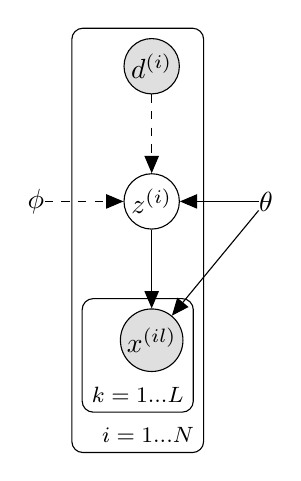
\begin{tikzpicture}[node distance = 1.5cm]
			\node[obs] (x) {$x^{(il)}$}; 
			
			\node[latent, above=of x] (z) {$z^{(i)}$}; 
			
			\node[obs, above=of z] (d) {$d^{(i)}$}; 
			
			\node[const, right=of z] (th) {$\theta$} ;
			\node[const, left=of z] (ph) {$\phi$};
			
			\edge {z} {x};
			\edge {th} {z};
			\edge {th} {x};
			
			\edge [dashed] {ph} {z}
			\edge [dashed] {d} {z}
			
			
			\plate {xz} {(x)} {$k = 1...L$};
			\plate {xzd} {(x)(z)(d)(xz)} {$i = 1...N$};
			
			\end{tikzpicture}
		\end{center}
		\caption{Graphical Model}
		\label{sgvb}
	\end{figure}
	
	
	\begin{figure}[ht]
		\begin{center}
			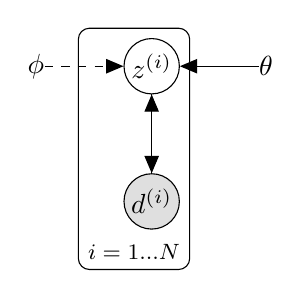
\begin{tikzpicture}[node distance = 1.5cm]
			
			
			\node[obs] (d) {$d^{(i)}$};
			
			\node[latent, above=of d] (z) {$z^{(i)}$};
			
			\node[const, right=of z] (th) {$\theta$} ;
			\node[const, left=of z] (ph) {$\phi$};
			
			
			\edge {z} {d};
			\edge {th} {z};
			\edge [dashed,bend left] {d} {z}
			\edge [dashed] {ph} {z}
			
			
			
			\plate {zd} {(z)(d)} {$i = 1...N$};
			
			\end{tikzpicture}
		\end{center}
		\caption{Graphical Model}
		\label{sgvb_dense}
	\end{figure}
	
	The graphical model we will use to model topics with SGVB is  equivalent to that of a VAE and is depicted in Figure (...). A notable difference from e.g. LDA \ref{lda_GM} is that we have one topic distribution for each document as opposed to each word in a document. This is much more practical for computational reasons, which we will discuss later. \\ \\
	
	Discuss implications of plate difference \\ \\
	
	Follow SGVB, but fill in specific model choices:  \\ 
	MLP as Encoder and Decoder, Gaussian latent variables with diagonal covariance, Multinomial output (and not Poisson as we don't want to model document length). Make objective function explicit. Discuss how interpretable the lowerbound is. 
	
	\section{Lower Bound}
	
	The log-likelihood of a data point i can be written as a sum of the lower bound and the KL divergence term between the true posterior $p(z|x,d)$ and the approximation $q(z|x,d)$, with $\theta$ the parameters of the model:
	
	\begin{align*}
	\log p(\mathbf{d}^{(i)}) = D_{KL}(q(\mathbf{z}^{(i)}|\mathbf{d}^{(i)}) || p(\mathbf{z}|\mathbf{d}^{(i)})) + \mathcal{L}(\mathbf{\theta}, \phi)
	\end{align*}
	
	We optimize the lowerbound: 
	
	\begin{align}
	%\mathcal{L}(\mathbf{\theta}, \phi; \mathbf{d}^{(i)}) = 
	%\mathbf{E}_{q_\phi} (\mathbf{z}|\mathbf{d}^{(i)})}[-\log
	%q_\ph	i (\mathbf{z}| \mathbf{d}^{(i)})+\log
	%p_\theta(\mathbf{z}^{(i)}|\mathbf{d}^{(i)}]
	\end{align}
	
	which, using Bayes rule, we can express as:
	
	\begin{align}
	\mathcal{L}(\mathbf{\theta}, \phi; \mathbf{d}^{(i)}) = -D_{KL}(q_\phi (\mathbf{z}| \mathbf{d}^{(i)})||_\theta (\mathbf{z})) + \mathbf{E}_{q_\phi(\mathbf{z}|\mathbf{d}^{(i)})}[\log p_\theta (\mathbf{d}^{(i)}|\mathbf{z})]
	\end{align}
	
	
	\section{KL Divergence}
	
	
	As in Kingma and Welling we can integrate the KL divergence analytically to obtain: \\
	
	
	\begin{align}
	- D_{KL}(q_\phi (\mathbf{z}| \mathbf{d})||p_\theta (\mathbf{z}| \mathbf{d})) = \frac{1}{2}\sum\limits_{j=1}^{J}\{1+\log \sigma_{\phi ,j}^2 - \mu_{\phi,j}^2 - \sigma_{\phi ,j}^2\}
	\end{align}
	
	Where $\mathbf{\mu}_\theta$ and $\mathbf{\sigma}_\theta^2$ represent the means and variances of the parametrized $p_\theta(\mathbf{z}|\mathbf{d})$.
	
	\section{Final objective function}
	
	An obvious choice for modelling the output distribution for count data would be Poisson. However, this also models the length of a document, which we do not expect to be very relevant for the topic. Therefore we use Multinomial probability for each word $x_n^{i}$ in document $d^{i}$. This way, we have that
	
	
	\begin{align}
	\log p_{\theta}(d^{(i)}|z^{(i)}) = 
	\sum_{n=1}^N
	\sum_{k=1}^K x_k^{(in)} \log (y_k^{(in)})
	\end{align}
	Where $k$ is the index of the output unit.\\
	
	
	Using a SGVB estimator, our final objective function consists of the negative KL divergence and the reconstruction error:
	
	\begin{align}
	\mathcal{L}(\mathbf{\theta}, \phi; \mathbf{d}^{(i)}) = \frac{1}{2}\sum\limits_{j=1}^{J}\{1+\log \sigma_{\phi ,j}^2 - \mu_{\phi,j}^2 - \sigma_{\phi ,j}^2\} 
	+ \sum_{n=1}^N
	\sum_{k=1}^K x_k^{(in)} \log (y_k^{(in)})
	\end{align}
	
	
	
	

	
	
	
	
\end{document}



	